\chapter{Introduction}

\section{Background}

Input your introduction here and here is the example of figures and tables.

\begin{itemize}
 \item	The example of citation:
	\cite{wu2024dynamic}
\item	The example of figure \autoref{fig:method}:
\item	The example of table \autoref{tab:notation}
\end{itemize}






\begin{figure*}[th]
	\centering
	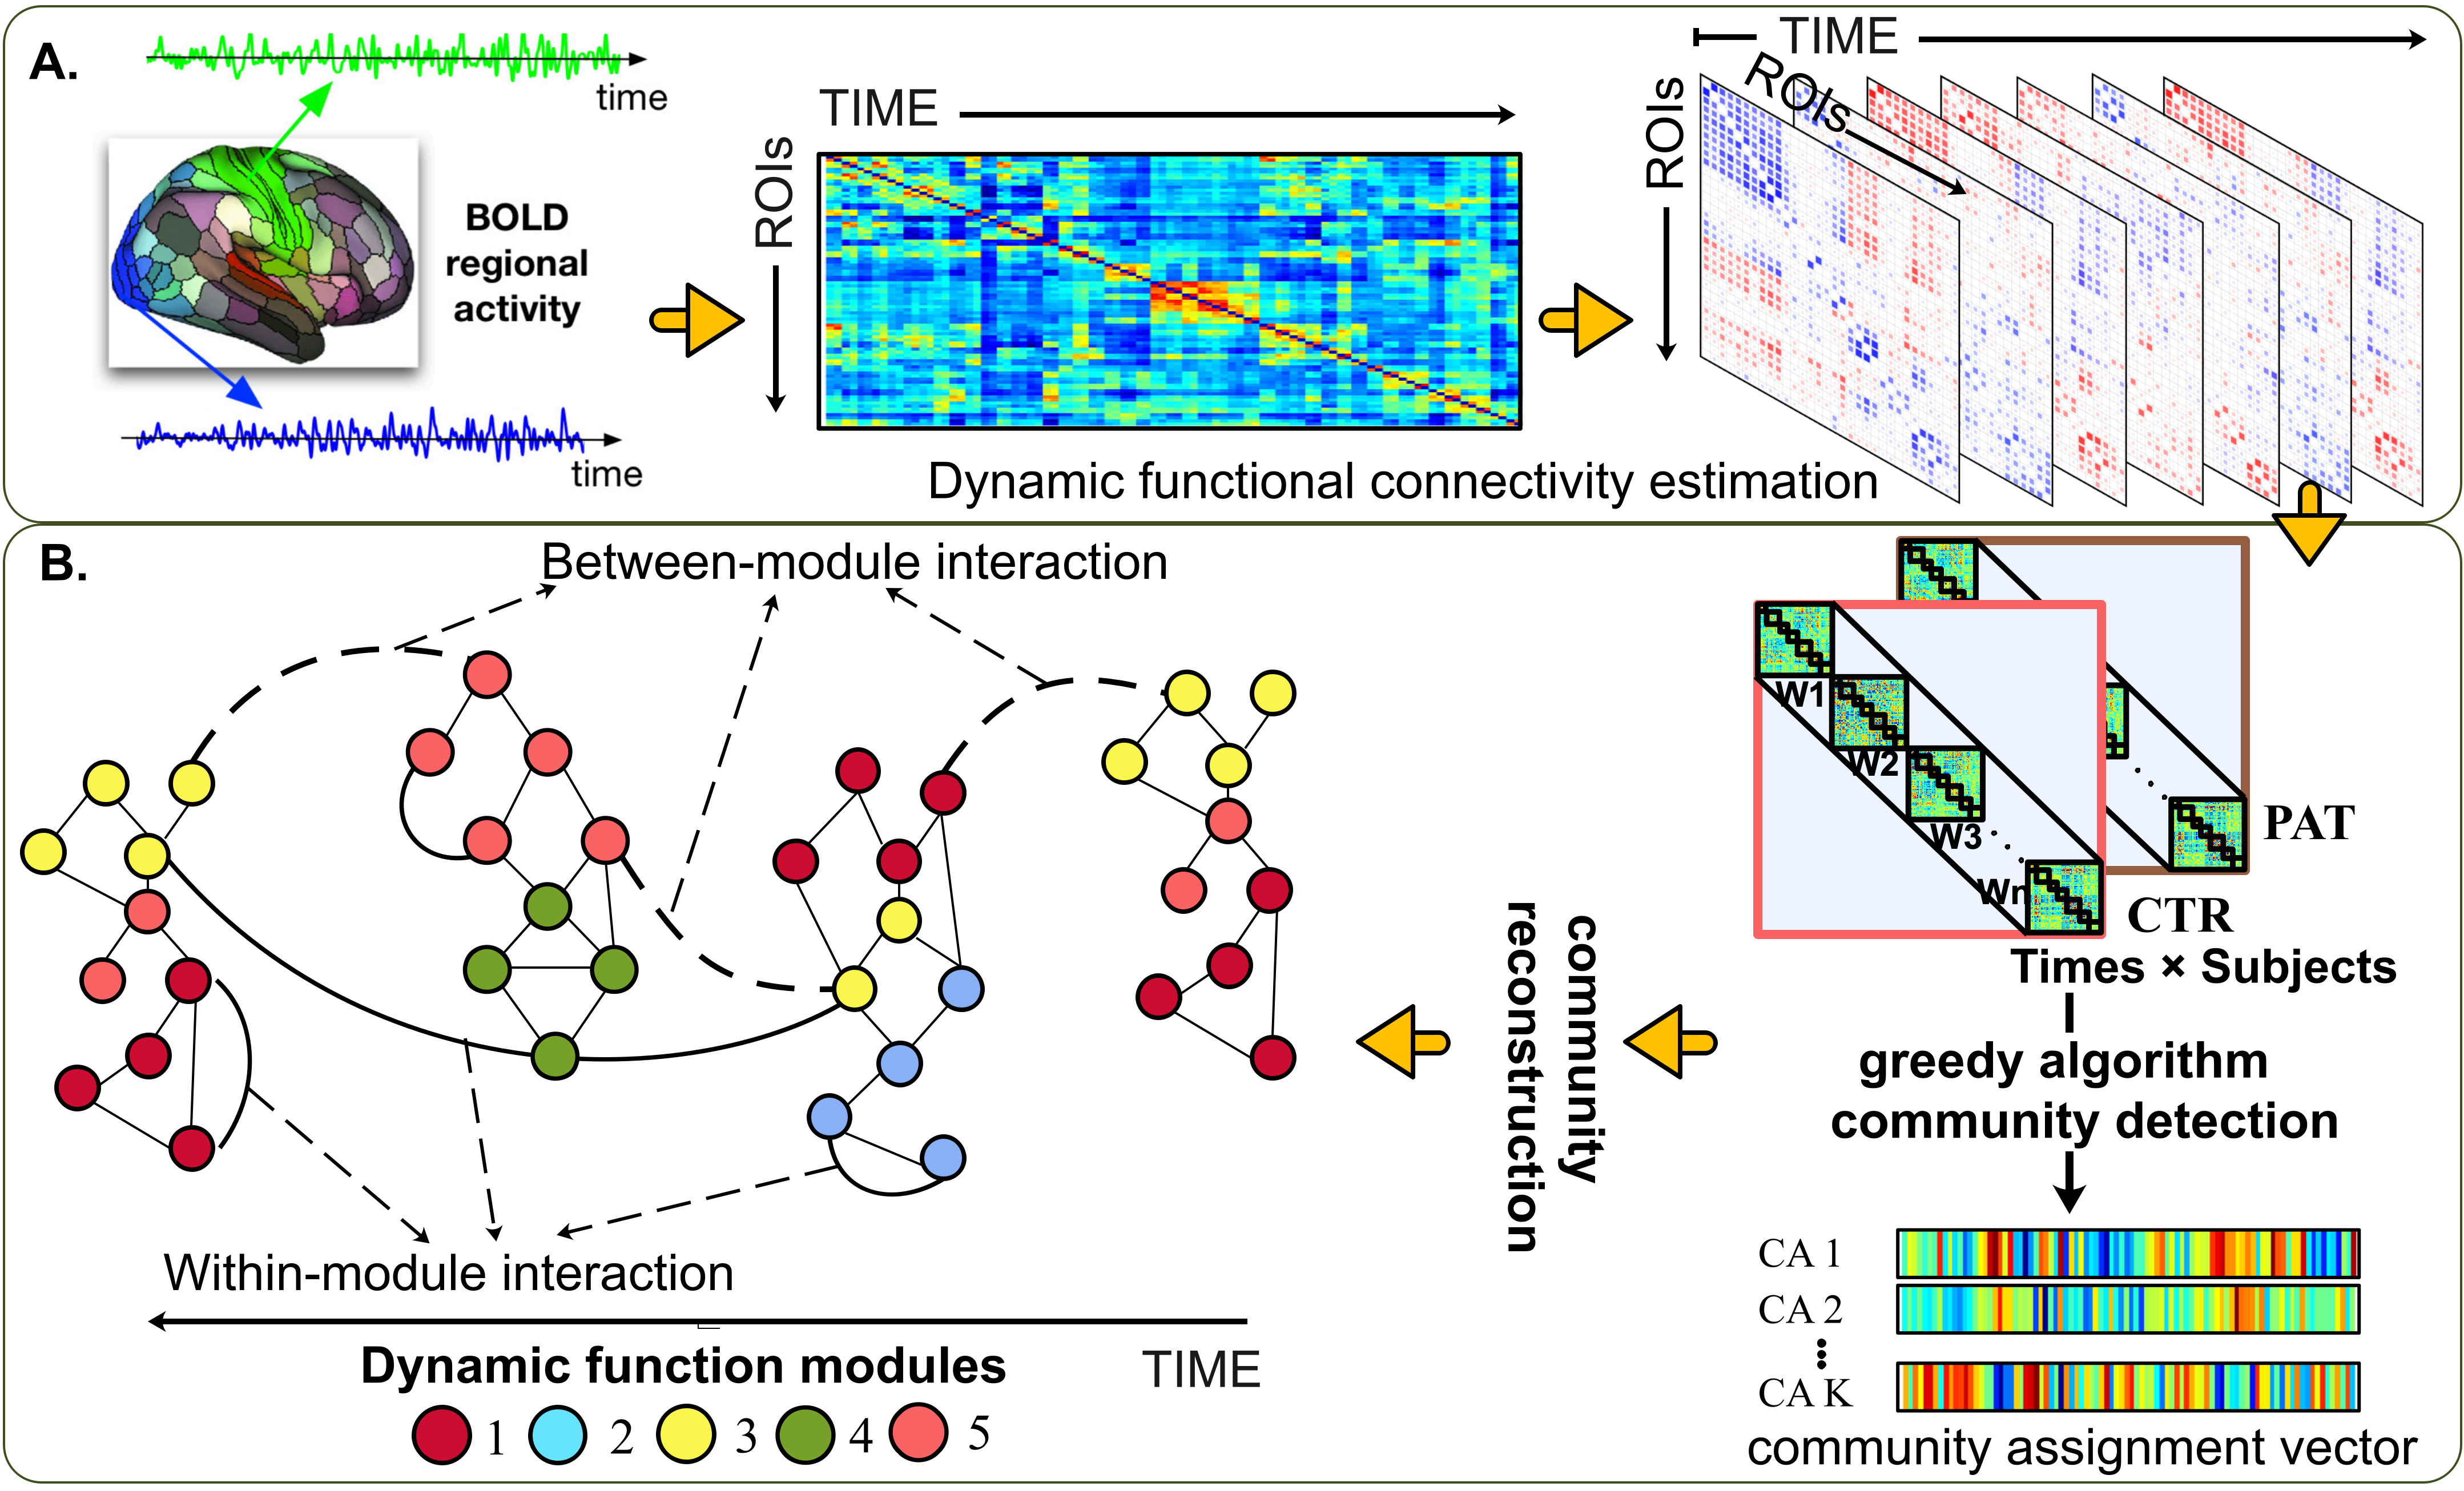
\includegraphics[width=0.8\textwidth]{Introduction/Pipeline.png}
	\caption{Flowchart of the proposed analytical framework.
		\textbf{A.} Dynamic functional connectivity estimation.
		\textbf{B.} Dynamic module interaction analysis. The arrows indicate the direction of data flow.
		\label{fig:method}}\vspace*{-2mm}
\end{figure*}


\begin{table*}
	\renewcommand\arraystretch{1.5}
	\setlength{\tabcolsep}{3pt}
	\centering
	\scriptsize
	\caption{Notation used in this chapter.}
	\label{tab:notation}
	\resizebox{\textwidth}{!}{
		\begin{tabular}{@{}clcl@{}}
			\toprule
			\textbf{Abbreviation} & \textbf{Definition} & \textbf{Abbreviation} & \textbf{Definition} 
			\\
			\midrule
			AIS & Acute Ischemic Stroke & 
			mRS & Modified Ranking Score \\
			
			AN & Auditory Network &
			MTG & Middle Temporal Gyrus \\
			
			ARAT & Action Research Arm Test &
			NIHSS & National Institutes of Health Stroke Scale  \\
			
			BOLD & Blood Oxygenation Level-Dependent &
			PCA & Principal Component Analysis \\
			
			DFC & Dynamic Functional Connectivity &
			PCC & Posterior Cingulate Cortex \\
			
			DLPFC & Dorsolateral Prefrontal Cortex &
			PMC & Premotor Cortex \\
			
			DMaaaN & Default Mode Network &
			PoCG & Postcentral Gyrus \\
			
			FC & Functional Connectivity &
			PPC & Posterior Parietal Cortex \\
			
			FCN & Functional Connectivity Network &
			PrG & Precentral Gyrus \\
			
			FMA & Fugel-Mayer Assessment &
			ROI & Region of Interest \\
			
			fMRI & Functional Magnetic Resonance Imaging &
			MPFC & Medial Prefrontal Cortex \\
			
			FNC & Functional Network Connectivity &
			SFC & Static Functional Connectivity \\
			
			HMM & Hidden Markov Model &
			SMA & Supplementary Motor Areas \\
			
			ICA & Independent Component Analysis &
			SMN & Sensorimotor Network \\
			
			M1 & Primary Motor Cortex &
			TD & Tensor Decomposition \\
			
			MFG & Middle Frontal Gyrus &
			WTC & Wavelet Transform Coherence \\
			
			%  & 
			% & & & & & \\
			\bottomrule
		\end{tabular}
	}
\end{table*}